\input{../utils/preamble}
\createdgmtitle{11}
%--------------------------------------------------------------------------------
\begin{document}
%--------------------------------------------------------------------------------
\begin{frame}
%\thispagestyle{empty}
\titlepage
\end{frame}
%=======
\begin{frame}{Recap of previous lecture}
	\begin{block}{Vanilla GAN}
		\vspace{-0.5cm}
		\[
			\min_{G} \max_D V(G, D) = \min_{G} \max_D \left[ \bbE_{\pi(\bx)} \log D(\bx) + \bbE_{p(\bz)} \log (1 - D(G(\bz))) \right]
		\]
		\vspace{-0.7cm}
	\end{block}
	\begin{block}{Main problems}
		\begin{itemize}
			\item Vanishing gradients (non-saturating GAN does not suffer of it);
			\item Mode collapse (caused by behaviour of Jensen-Shannon divergence).
		\end{itemize}
	\end{block}
	\vspace{-0.1cm}
	\begin{block}{Informal theoretical results}
		Distribution of real images $\pi(\bx)$ and distribution of generated images $p(\bx | \btheta)$ are low-dimensional and have disjoint supports. In this case
		\vspace{-0.3cm}
		\[
			KL(\pi || p) = KL(p || \pi) = \infty, \quad JSD(\pi || p) = \log 2
		\]
		\end{block}
		\myfootnote{\href{https://arxiv.org/abs/1406.2661}{Goodfellow I. J. et al. Generative Adversarial Networks, 2014} \\
		\href{https://arxiv.org/abs/1701.04862}{Arjovsky M., Bottou L. Towards Principled Methods for Training Generative Adversarial Networks, 2017}}
\end{frame}
%=======
\begin{frame}{Recap of previous lecture}
		\begin{block}{Wasserstein distance}
			\vspace{-0.5cm}
			\[
				W(\pi, p) = \inf_{\gamma \in \Gamma(\pi, p)} \bbE_{(\bx, \by) \sim \gamma} \| \bx - \by \| =  \inf_{\gamma \in \Gamma(\pi, p)} \int \| \bx - \by \| \gamma (\bx, \by) d \bx d \by
			\]
			\vspace{-0.5cm}
			\begin{itemize}
				\item $\Gamma(\pi, p)$ -- the set of all joint distributions $\Gamma (\bx, \by)$ with marginals $\pi$ and $p$ ($\int \gamma(\bx, \by) d \bx = p(\by)$, $\int \gamma(\bx, \by) d \by = \pi(\bx)$)
				\item $\gamma(\bx, \by)$ -- transportation plan (the amount of "dirt" that should be transported from point $\bx$ to point $\by$).
				\item $\gamma(\bx, \by)$ -- the amount, $\|\bx - \by \|$-- the distance.
			\end{itemize}
		\end{block}
		\begin{block}{Kantorovich-Rubinstein duality}
			\vspace{-0.2cm}
			\[
				W(\pi || p) = \frac{1}{K} \max_{\| f \|_L \leq K} \left[ \bbE_{\pi(\bx)} f(\bx)  - \bbE_{p(\bx)} f(\bx)\right],
			\]
			where $\| f \|_L \leq K$ are $K-$Lipschitz continuous functions ($f: \cX \rightarrow \bbR$).
		\end{block}
		\myfootnotewithlink{https://arxiv.org/abs/1701.07875}{Arjovsky M., Chintala S., Bottou L. Wasserstein GAN, 2017}
\end{frame}
%=======
\begin{frame}{Recap of previous lecture}
		\begin{block}{Vanilla GAN objective}
			\vspace{-0.2cm}
			\[
				\min_{G} \max_D \bbE_{\pi(\bx)} \log D(\bx) + \bbE_{p(\bz)} \log (1 - D(G(\bz)))
			\]
			\vspace{-0.2cm}
		\end{block}
		\begin{block}{WGAN objective}
			\vspace{-0.6cm}
			\[
			\min_{G} W(\pi || p) = \min_{G} \max_{\bphi \in \boldsymbol{\Phi}} \left[ \bbE_{\pi(\bx)} f(\bx, \bphi)  - \bbE_{p(\bz)} f(G(\bz), \bphi )\right].
			\]
		\end{block}
		\begin{itemize}
			\item Discriminator $D$ is similar to the function $f$, but not the same (it is not a classifier anymore). In the WGAN model, function~$f$ is usually called $\textit{critic}$.
			\item "Weight clipping is a clearly terrible way to enforce a Lipschitz constraint". If the clipping parameter is large, it is hard to train the critic till optimality. If the clipping parameter is too small, it could lead to vanishing gradients.
		\end{itemize}
		\myfootnotewithlink{https://arxiv.org/abs/1701.07875}{Arjovsky M., Chintala S., Bottou L. Wasserstein GAN, 2017}
		
\end{frame}
%=======
\begin{frame}{Wasserstein GAN with Gradient Penalty}
	\begin{block}{Weight clipping annalysis}
		\begin{itemize}
			\item The critic ignores higher moments of the data distribution.
			\item The gradients either grow or decay exponentially.
		\end{itemize}
	\end{block}
	\vspace{-0.2cm}
	\begin{figure}
		\centering
		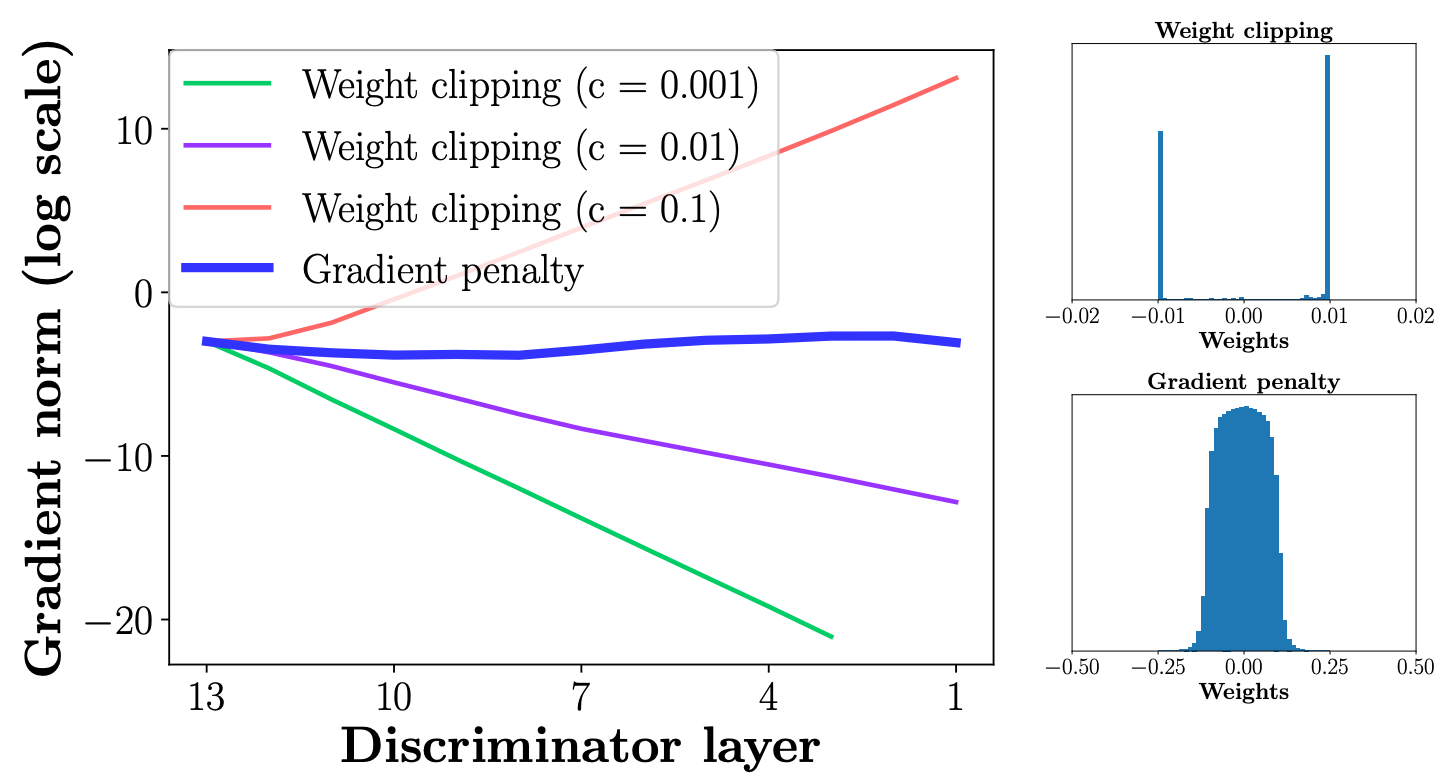
\includegraphics[width=0.8\linewidth]{figs/wgan_gp_weights}
	\end{figure}
	\vspace{-0.2cm} 
	
	Gradient penalty makes the gradients  more stable.
	\myfootnotewithlink{https://arxiv.org/abs/1704.00028}{Gulrajani I. et al. Improved Training of Wasserstein GANs, 2017}
\end{frame}
%=======
\begin{frame}{Wasserstein GAN with Gradient Penalty}
	\begin{block}{Theorem}
		Let $\pi(\bx)$ and $p(\bx)$ be two distribution in $\cX$, a compact metric space. Then, there is 1-Lipschitz function $f^*$ which is the optimal solution of 
		\[
			\max_{\| f \|_L \leq 1} \left[ \bbE_{\pi(\bx)} f(\bx)  - \bbE_{p(\bx)} f(\bx)\right].
		\]
		Let $\gamma$ be the optimal transportation plan between $\pi(\bx)$ and $p(\bx)$. Then, if $f^*$ is differentiable, $\gamma(\bx = \by) = 0$ and $\hat{\bx}_t = t \bx + (1 - t) \by$ with $t \in [0, 1]$ it holds that
		\[
			\bbP_{(\bx, \by) \sim \gamma} \left[ \nabla f^*(\hat{\bx}_t) = \frac{\by - \hat{\bx}_t}{\| \by - \hat{\bx}_t \|} \right] = 1.
		\]
	\end{block}
	\vspace{-0.2cm}
	\begin{block}{Corollary}
		$f^*$ has gradient norm 1 almost everywhere under $\pi(\bx)$ and $p(\bx)$.
	\end{block}

	\myfootnotewithlink{https://arxiv.org/abs/1704.00028}{Gulrajani I. et al. Improved Training of Wasserstein GANs, 2017}
\end{frame}
%=======
\begin{frame}{Wasserstein GAN with Gradient Penalty}
	A differentiable function is 1-Lipschtiz if and only if it has gradients with norm at most 1 everywhere.
	\begin{block}{Gradient penalty}
		\[
			W(\pi || p) = \underbrace{\bbE_{\pi(\bx)} f(\bx)  - \bbE_{p(\bx)} f(\bx)}_{\text{original critic loss}} + \lambda \underbrace{\bbE_{\hat{\bx}} \left[ \left( \| \nabla_{\hat{\bx}} f(\hat{\bx}) \|_2 - 1 \right) ^ 2\right]}_{\text{gradient penalty}},
		\]
	\end{block}
	\begin{itemize}
		\item Samples $\hat{\bx}$ are uniformly sampled along straight lines between pairs of points from the data distribution $\pi(\bx)$ and the generator distribution $p(\bx | \btheta)$.
		\item Enforcing the unit gradient norm constraint everywhere is intractable, it turns out to be sifficient to enforce it only along these straight lines.
	\end{itemize}

	\myfootnotewithlink{https://arxiv.org/abs/1704.00028}{Gulrajani I. et al. Improved Training of Wasserstein GANs, 2017}
\end{frame}
%=======
\begin{frame}{Wasserstein GAN with Gradient Penalty}
	
	\begin{figure}
		\centering
		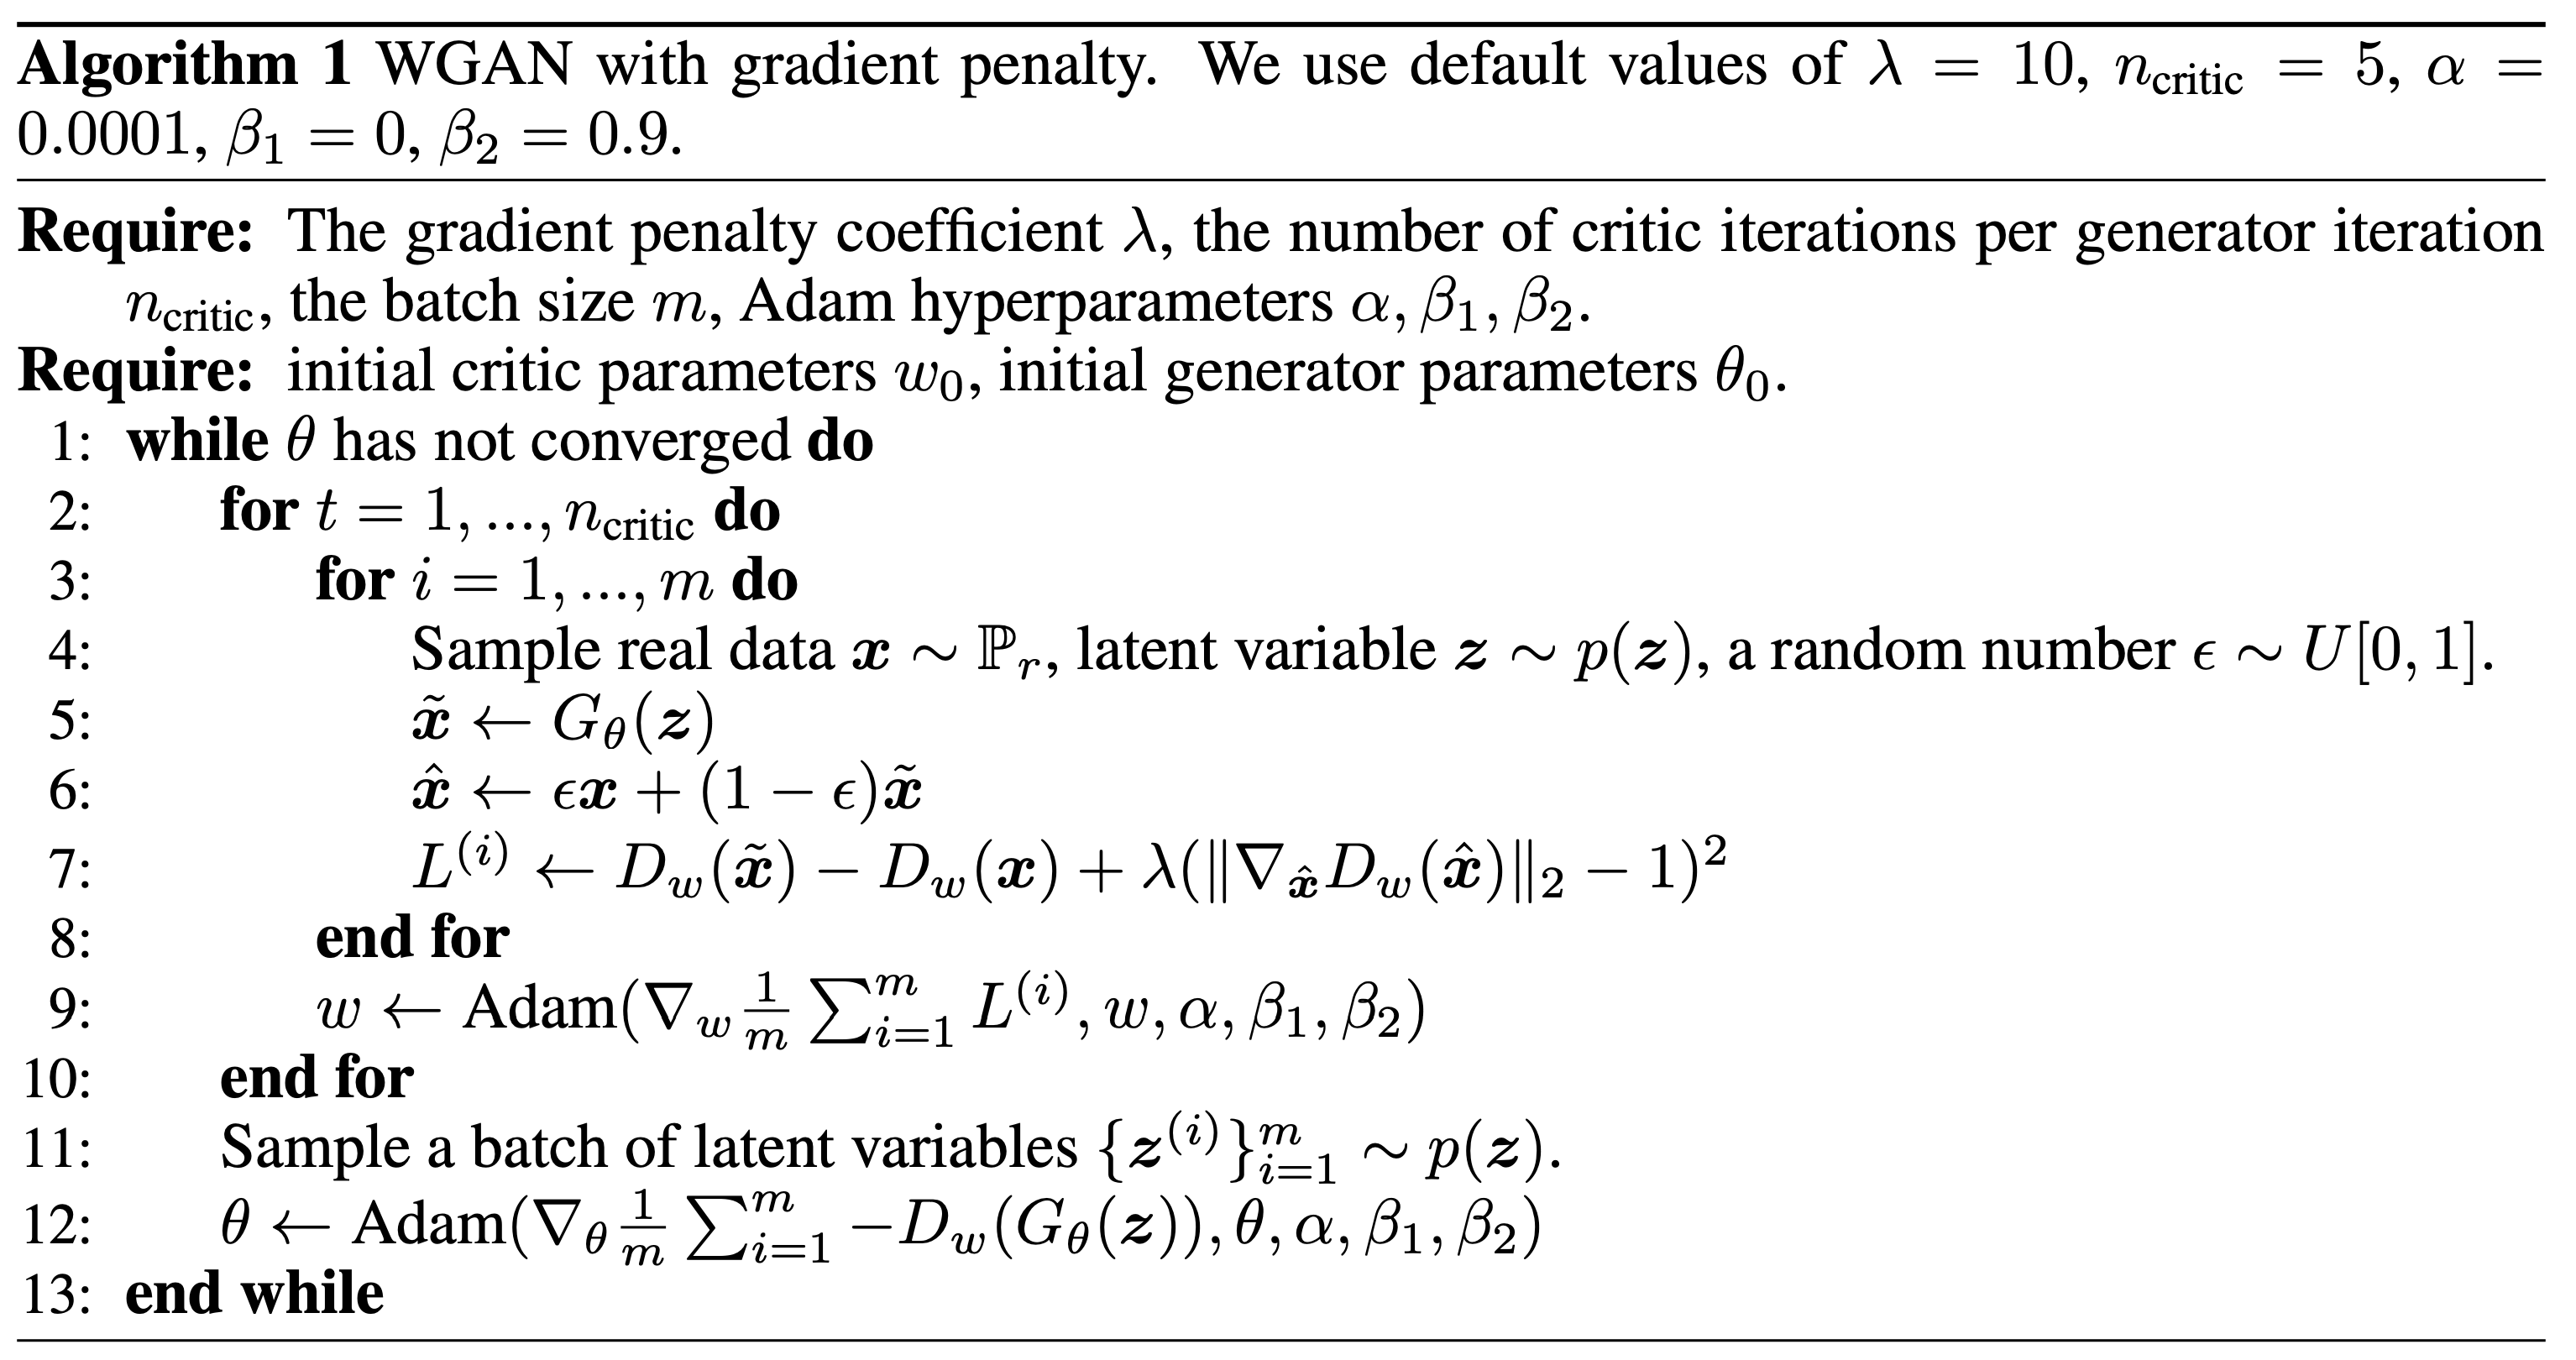
\includegraphics[width=1.0\linewidth]{figs/wgan_gp_pseudocode}
	\end{figure}

	\myfootnotewithlink{https://arxiv.org/abs/1704.00028}{Gulrajani I. et al. Improved Training of Wasserstein GANs, 2017}
\end{frame}
%=======
\begin{frame}{Wasserstein GAN with Gradient Penalty}
	\begin{figure}
		\centering
		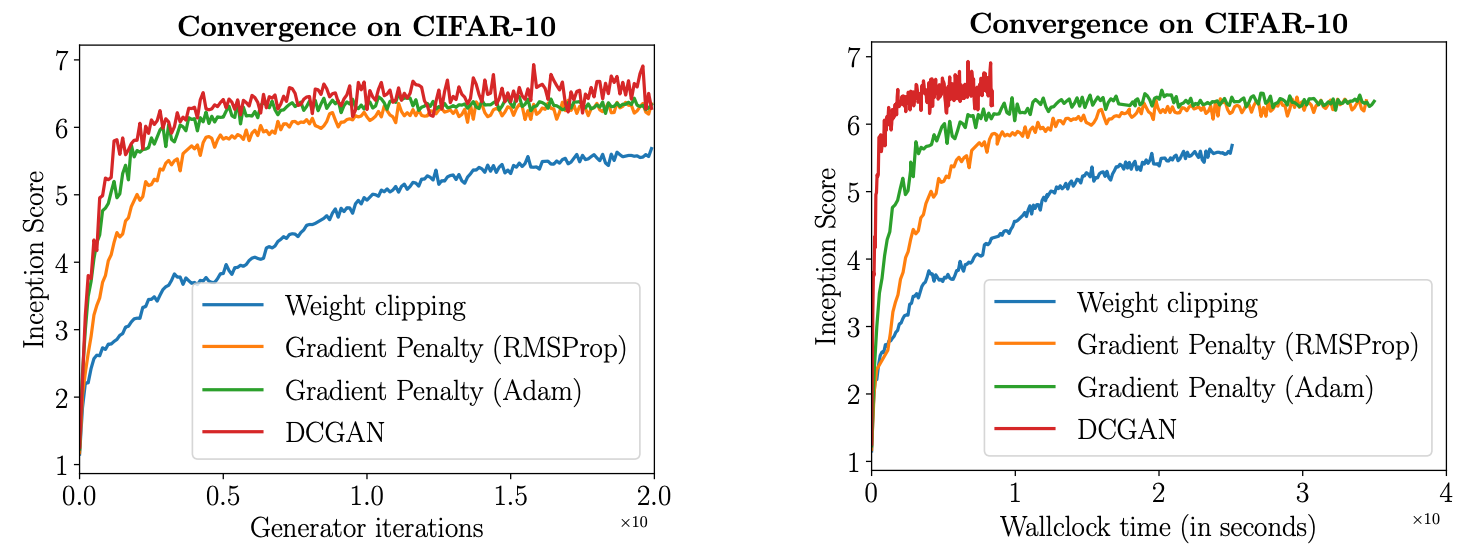
\includegraphics[width=\linewidth]{figs/wgan_gp_convergence}
	\end{figure}
	\begin{figure}
		\centering
		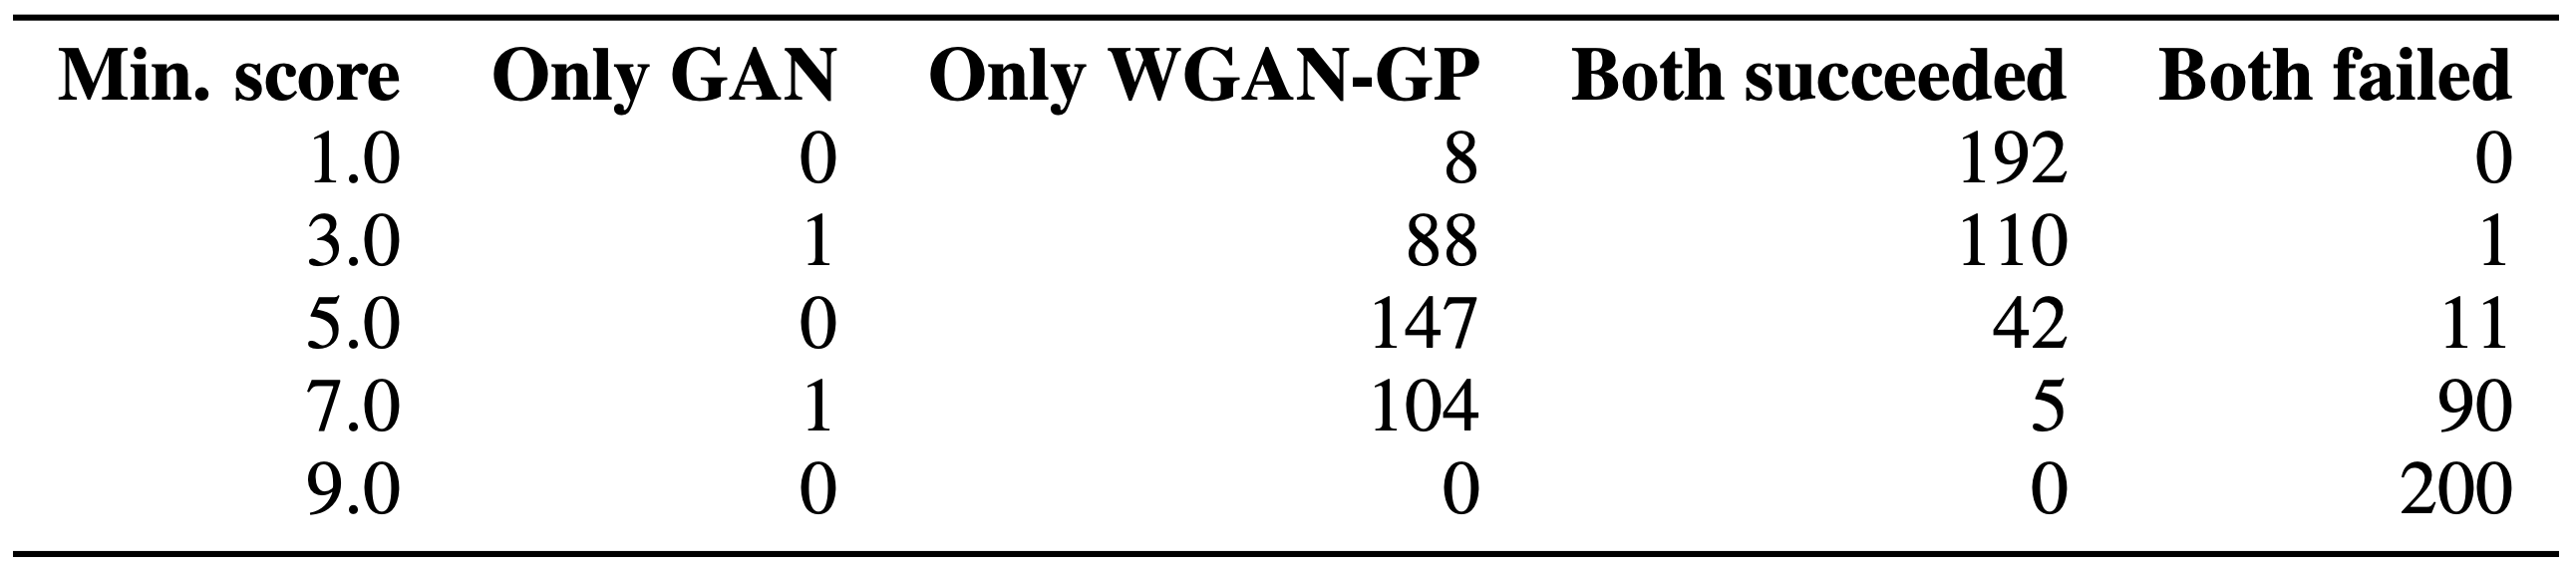
\includegraphics[width=0.75\linewidth]{figs/wgan_gp_wgan}
	\end{figure}

	\myfootnotewithlink{https://arxiv.org/abs/1704.00028}{Gulrajani I. et al. Improved Training of Wasserstein GANs, 2017}
\end{frame}
%=======
\begin{frame}{Wasserstein GAN with Gradient Penalty}
	\begin{figure}
		\centering
		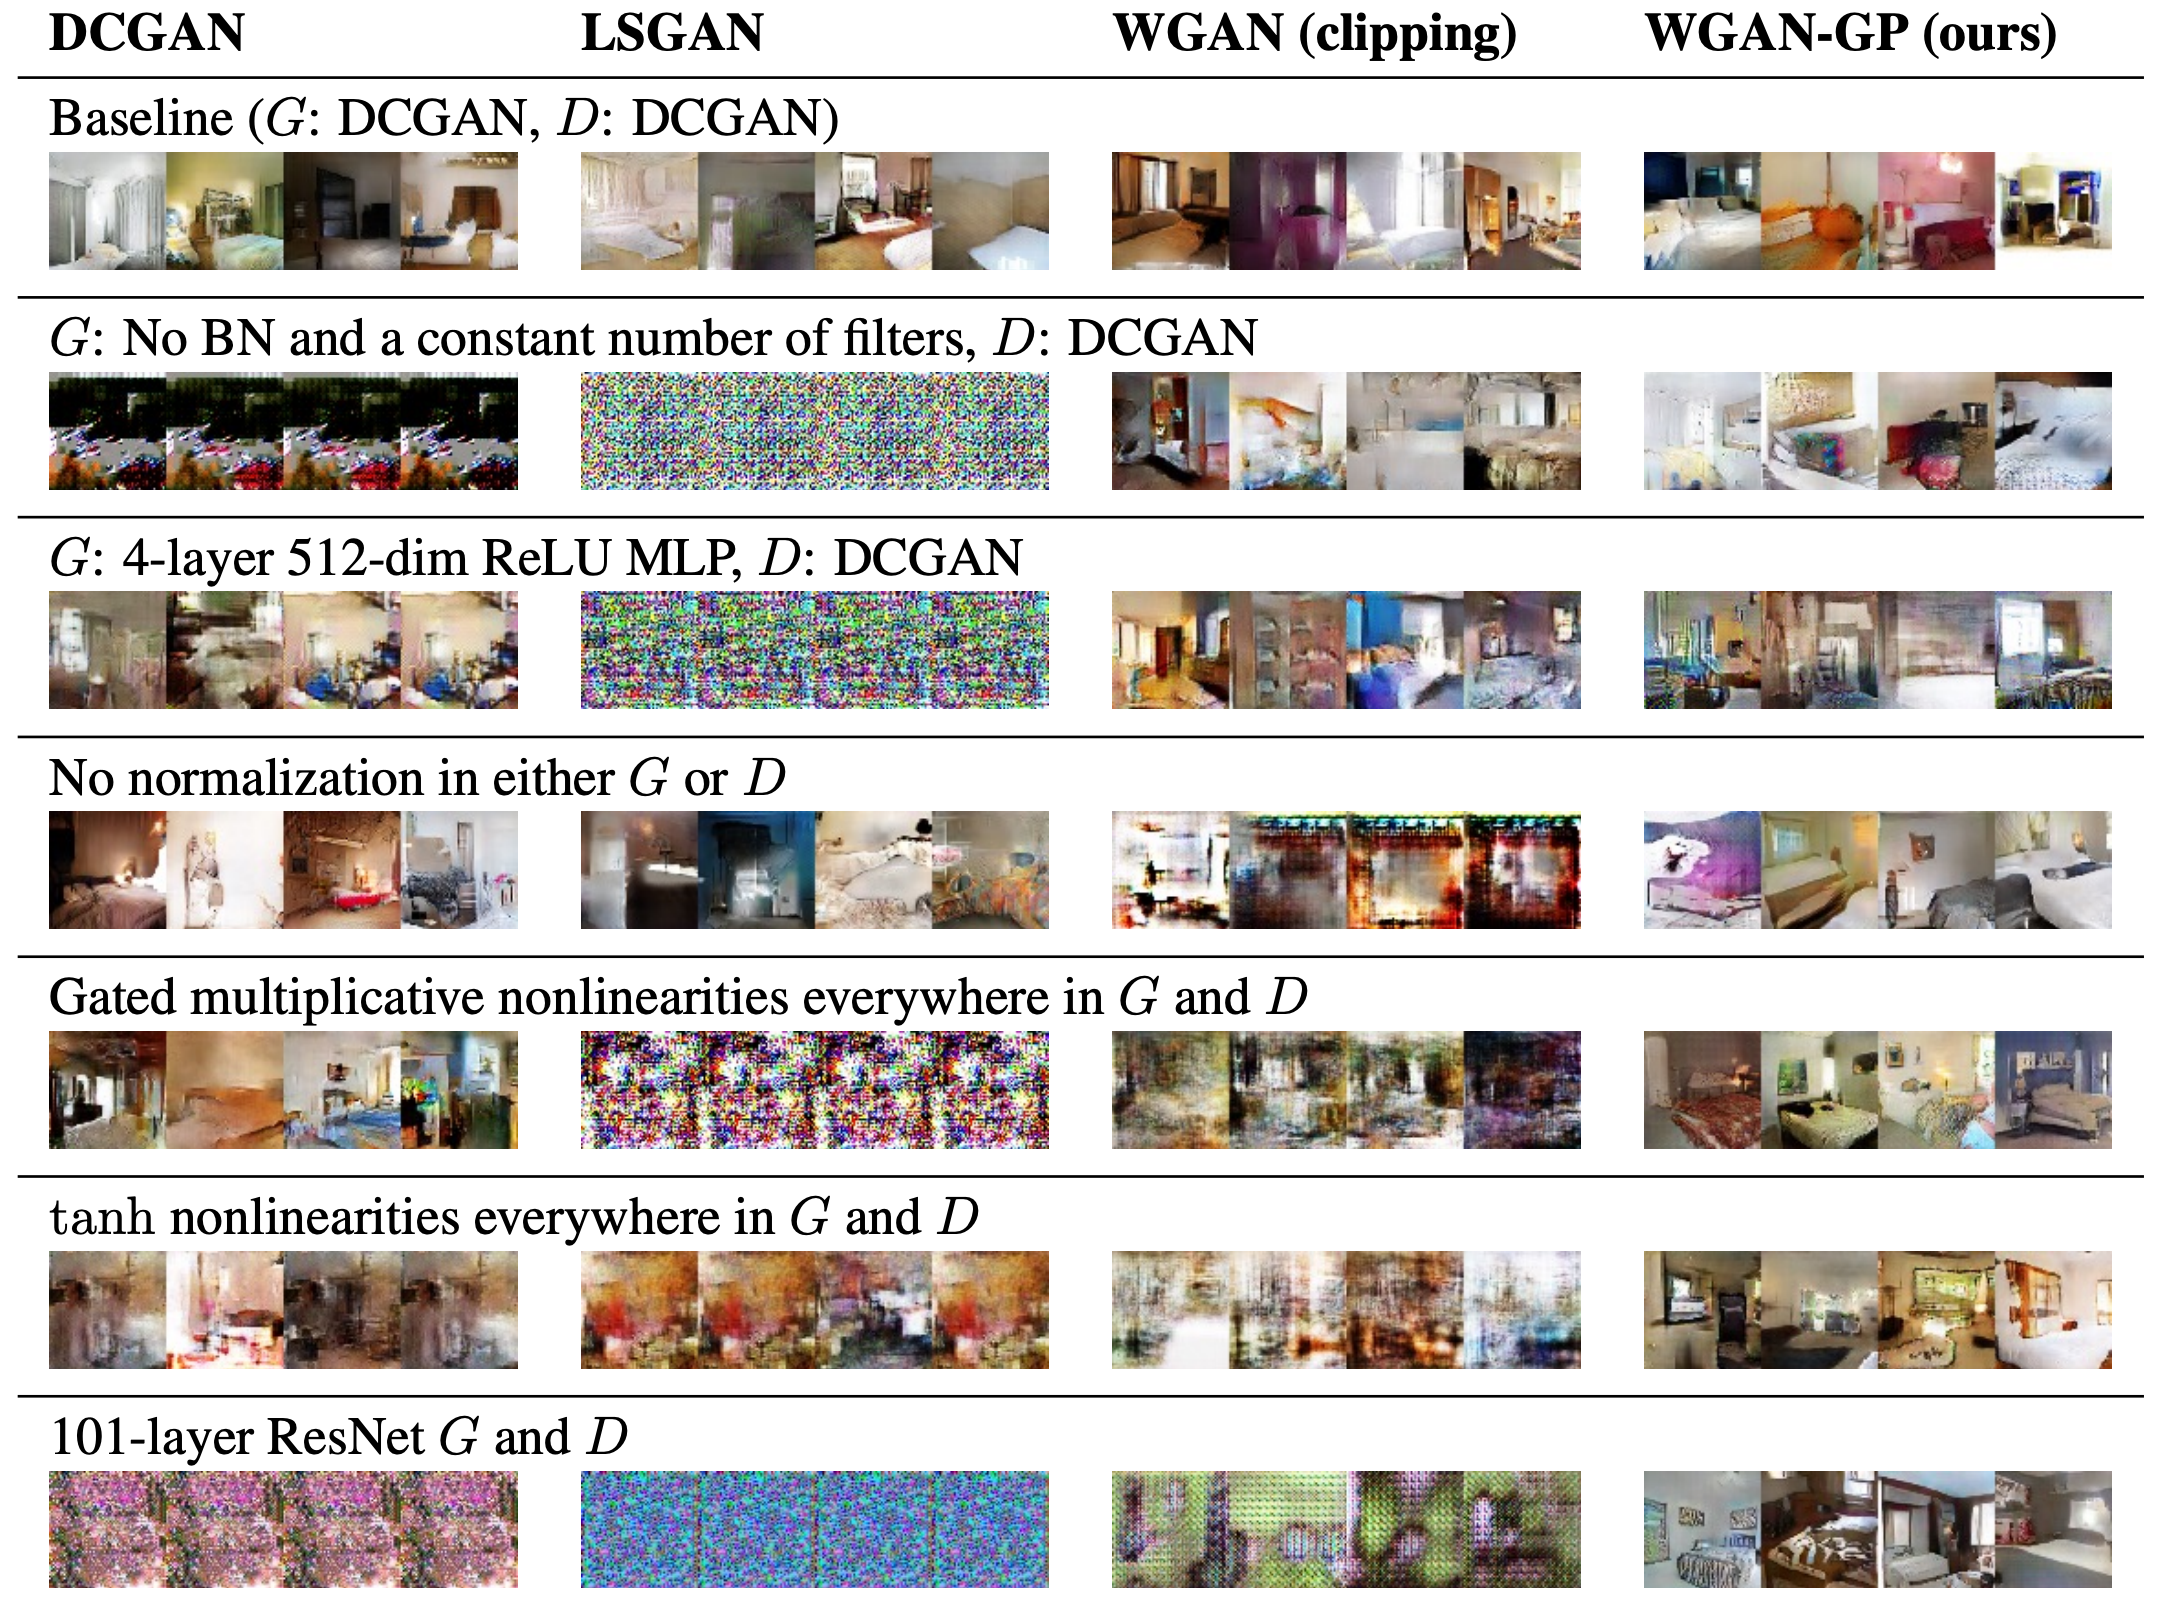
\includegraphics[width=0.95\linewidth]{figs/wgan_gp_results}
	\end{figure}

	\myfootnotewithlink{https://arxiv.org/abs/1704.00028}{Gulrajani I. et al. Improved Training of Wasserstein GANs, 2017}
\end{frame}
%=======
\begin{frame}{Spectral Normalization GAN}
	How else could we enforce Lipschitzness?
	\begin{block}{Fact 1}
		Let denote by $\sigma(\bA)$ a spectral norm of matrix $\bA$.
		\[
			\sigma(\bA) = \max_{\bh \neq 0} \frac{\|\bA \bh\|_2}{\|\bh\|_2} = \max_{\|\bh\|_2 \leq 1} \| \bA \bh \|_2 = \lambda_{\text{max}}(\bA),
		\]
		where $\lambda_{\text{max}}(\bA)$ is the largest singular value of $\bA$. \\
		By definition, Lipschitz norm is 
		\[
			\| \mathbf{g} \|_L = \sup_\bx \sigma( \nabla \mathbf{g}(\bx))
		\]
	\end{block}
	\vspace{-0.5cm}
	\begin{block}{Fact 2}
		Lipschitz norm of superposition is bounded above by product of Lipschitz norms
		\vspace{-0.2cm}
		\[
			\| \mathbf{g}_1 \circ \mathbf{g}_2 \|_L \leq \| \mathbf{g}_1 \|_L \cdot \| \mathbf{g}_2\|_L
		\]
	\end{block}
	\myfootnotewithlink{https://arxiv.org/abs/1802.05957}{Miyato T. et al. Spectral Normalization for Generative Adversarial Networks, 2018}
\end{frame}
%=======
\begin{frame}{Spectral Normalization GAN}
	Let consider the critic $f(\bx, \bphi)$ of the following form:
	\[
		f(\bx, \bphi) = \bW_{K+1} a_K (\bW_K a_{K-1}(\dots a_1(\bW_1 \bx) \dots)).
	\]
	This feedforward network is a superposition of simple functions.
	\begin{itemize}
		\item $a_k$ is a pointwise nonlinearities. We assume that $\| a_k \|_L = 1$ (it holds for ReLU).
		\item $\mathbf{g}(\bh) = \bW \bh$ is a linear transformation ($\nabla \mathbf{g}(\bx) = \bW$).
		\[
			\| \mathbf{g} \|_L = \sup_\bx \sigma( \nabla \mathbf{g}(\bx)) = \sigma(\bW).
		\]
	\end{itemize}
	\vspace{-0.3cm}
	\begin{block}{Critic spectral norm}
		\vspace{-0.3cm}
		\[
			\| f \|_L \leq \| \bW_{K+1}\| \cdot \prod_{k=1}^K  \| a_k \|_L \cdot \| \bW_k \| = \prod_{k=1}^{K+1} \sigma(\bW_k).
		\]
		\vspace{-0.2cm}
	\end{block}
	If we replace the weights in the critic $f(\bx, \bphi)$ by $\bW^{SN}_k = \bW_k / \sigma(\bW_k)$, we will get $\| f\|_L \leq 1.$ \\
	
	\myfootnotewithlink{https://arxiv.org/abs/1802.05957}{Miyato T. et al. Spectral Normalization for Generative Adversarial Networks, 2018}
\end{frame}
%=======
\begin{frame}{Spectral Normalization GAN}
	How to compute $\sigma(\bW)$? \\
	 If we apply singular value decomposition to compute the $\sigma(\bW)$ at each round of the algorithm, the algorithm becomes intractable.
	 
	 \begin{block}{Power iteration}
	 	\begin{itemize}
	 		\item $\bu_0$ -- random vector.
	 		\item for $k = 0, \dots, n - 1$: ($n$ is a large enough number of steps)
	 		\[
	 			\bv_{k+1} = \frac{\bW^T \bu_{k}}{\| \bW^T \bu_{k} \|}, \quad \bu_{k+1} = \frac{\bW \bv_{k+1}}{\| \bW \bv_{k+1} \|}
	 		\]
	 		\item approximate the spectral norm
	 		\[
	 			\sigma(\bW) \approx \bu_{n}^T \bW \bv_{n}
	 		\]
	 	\end{itemize}
	 \end{block}

	\myfootnotewithlink{https://arxiv.org/abs/1802.05957}{Miyato T. et al. Spectral Normalization for Generative Adversarial Networks, 2018}
\end{frame}
%=======
\begin{frame}{Spectral Normalization GAN}
	\begin{figure}
		\centering
		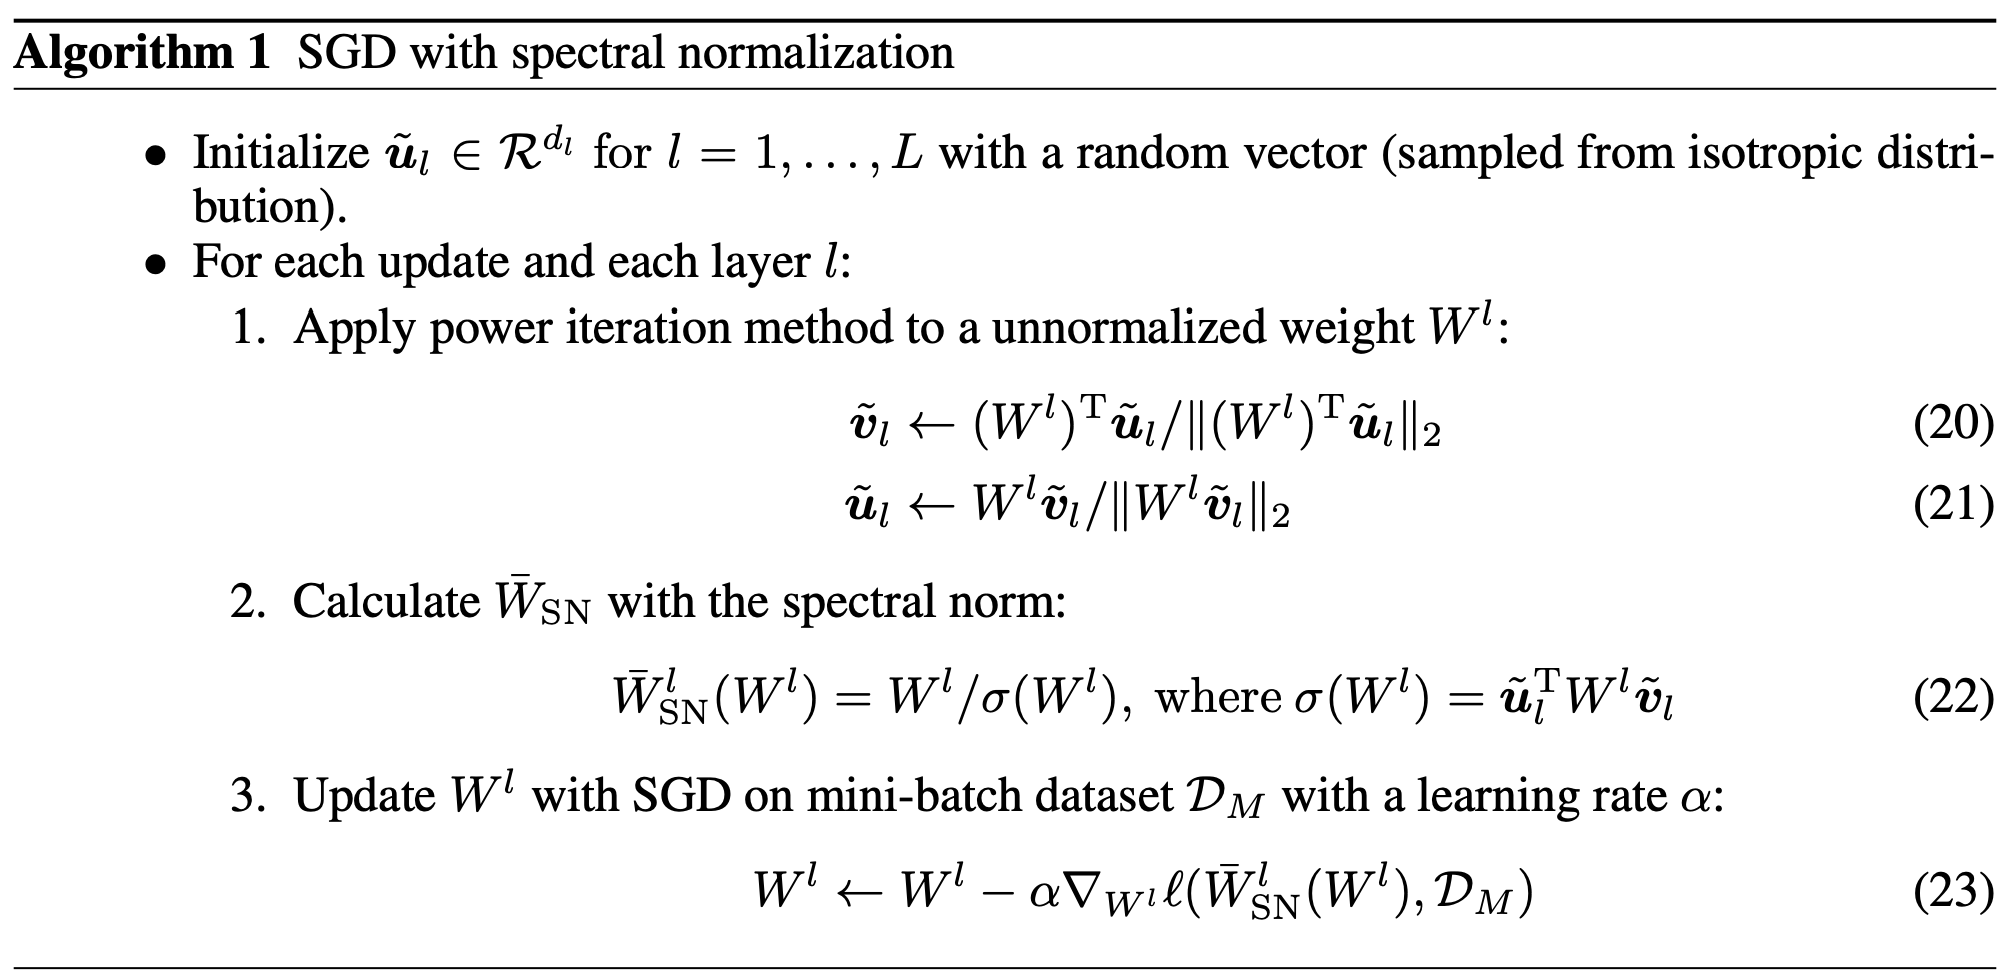
\includegraphics[width=0.85\linewidth]{figs/sngan_pseudocode}
	\end{figure}
	\begin{figure}
		\centering
		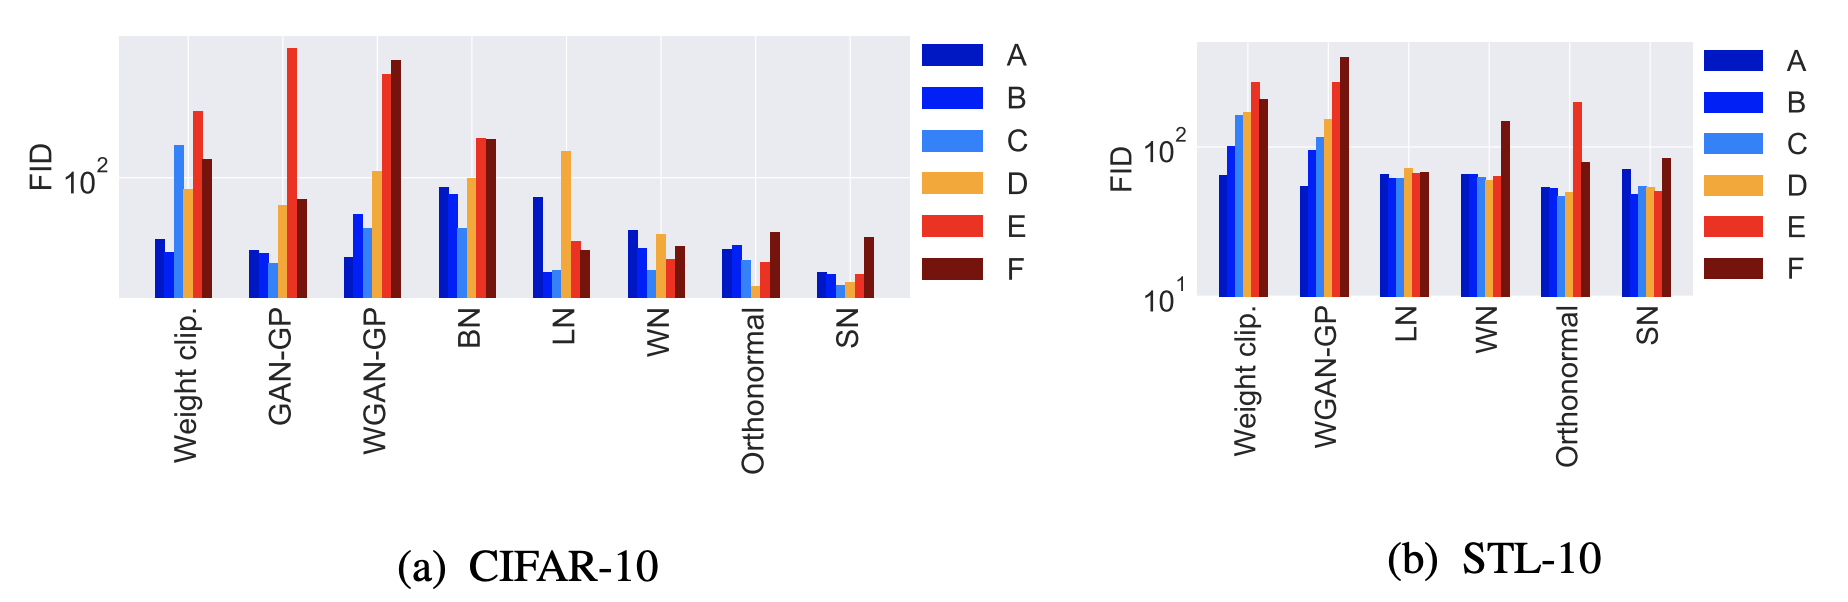
\includegraphics[width=0.85\linewidth]{figs/sngan_fids}
	\end{figure}

	\myfootnotewithlink{https://arxiv.org/abs/1802.05957}{Miyato T. et al. Spectral Normalization for Generative Adversarial Networks, 2018}
\end{frame}
%=======
\begin{frame}{Divergences}
	\begin{block}{What do we have?}
		\begin{itemize}
			\item Forward KL divergence in maximum likelihood estimation
			\item Reverse KL in variational inference
			\item JS divergence in  vanilla gan
			\item Wasserstein distance in WGAN
		\end{itemize}
	\end{block}
	\begin{block}{What is a divergence?}
		Let $\cS$ be the set of all possible probability distributions. Then $D: \cS \times \cS \rightarrow \bbR$ is a divergence if 
		\begin{itemize}
			\item $D(\pi || p) \geq 0$ for all $\pi, p \in \cS$;
			\item $D(\pi || p) = 0$ if and only if $\pi \equiv p$.
		\end{itemize}
	\end{block}
	\begin{block}{General divergence minimization task}
		\vspace{-0.3cm}
		\[
			\min_p D(\pi || p)
		\]
		\vspace{-0.5cm}
	\end{block}
\end{frame}
%=======
\begin{frame}{f-divergence family}
	
	\begin{block}{f-divergence}
		\vspace{-0.3cm}
		\[
		D_f(\pi || p) = \bbE_{p(\bx)}  f\left( \frac{\pi(\bx)}{p(\bx)} \right)  = \int p(\bx) f\left( \frac{\pi(\bx)}{p(\bx)} \right) d \bx.
		\]
		Here $f: \bbR_+ \rightarrow \bbR$ is a convex, lower semicontinuous function satisfying $f(1) = 0$.
	\end{block}
	\begin{figure}
		\centering
		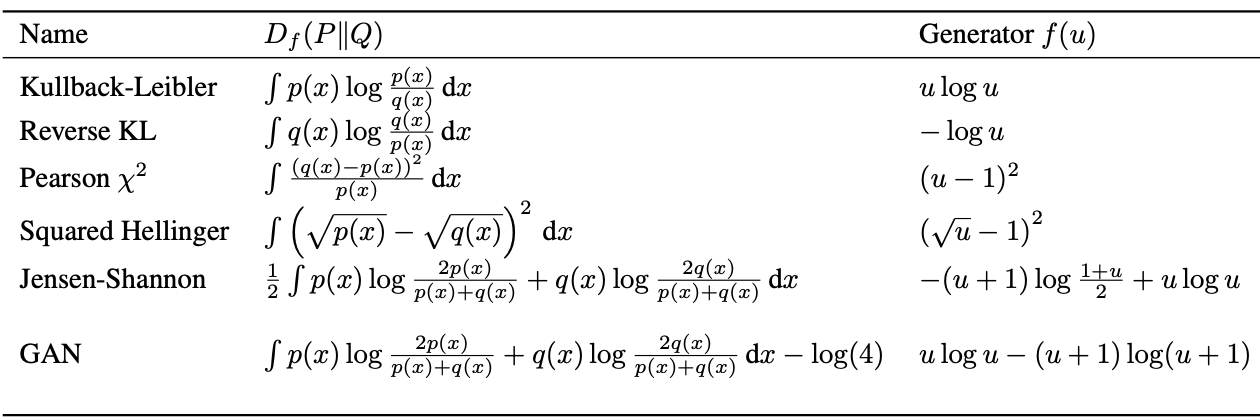
\includegraphics[width=\linewidth]{figs/f_divs}
	\end{figure}
	\myfootnotewithlink{https://arxiv.org/abs/1606.00709}{Nowozin S., Cseke B., Tomioka R. f-GAN: Training Generative Neural Samplers using Variational Divergence Minimization, 2016}
\end{frame}
%=======
\begin{frame}{f-divergence family}
	\vspace{-0.2cm}
	\begin{block}{Fenchel conjugate}
		\vspace{-0.7cm}
		\[
		f^*(t) = \sup_{u \in \text{dom}_f} \left( ut - f(u) \right), \quad f(u) = \sup_{t \in \text{dom}_{f^*}} \left( ut - f^*(t) \right)
		\]
		\vspace{-0.5cm}
	\end{block}
	\textbf{Important property:} $ f^{**} = f$ for convex $f$.
	\begin{block}{f-divergence}
		\vspace{-0.8cm}
		\begin{multline*}
			D_f(\pi || p) = \bbE_{p(\bx)}  f\left( \frac{\pi(\bx)}{p(\bx)} \right)  = \int p(\bx) f\left( \frac{\pi(\bx)}{p(\bx)} \right) d \bx = \\ = \int p(\bx) \sup_{t \in \text{dom}_{f^*}} \left( \frac{\pi(\bx)}{p(\bx)} t - f^*(t) \right) d \bx = \\ 
			= \int \sup_{t \in \text{dom}_{f^*}} \left( \pi(\bx)t - p(\bx) f^*(t) \right) d \bx .
		\end{multline*}
		\vspace{-0.6cm}
	\end{block}
	Here we seek value of $t$, which gives us maximum value of $ \pi(\bx)t - p(\bx) f^*(t)$, for each data point $\bx$.
	\myfootnotewithlink{https://arxiv.org/abs/1606.00709}{Nowozin S., Cseke B., Tomioka R. f-GAN: Training Generative Neural Samplers using Variational Divergence Minimization, 2016}
\end{frame}
%=======
\begin{frame}{f-divergence family}
	\vspace{-0.4cm}
	\begin{block}{f-divergence}
		\vspace{-0.3cm}
		\[
		D_f(\pi || p) = \bbE_{p(\bx)}  f\left( \frac{\pi(\bx)}{p(\bx)} \right)  = \int p(\bx) f\left( \frac{\pi(\bx)}{p(\bx)} \right) d \bx.
		\]
		\vspace{-0.4cm}
	\end{block}
	\begin{block}{Variational f-divergence estimation}
		\vspace{-0.8cm}
		\begin{multline*}
			D_f(\pi || p)  = \int \sup_{t \in \text{dom}_{f^*}} \left( \pi(\bx)t - p(\bx) f^*(t) \right) d \bx \geq \\
			 \geq \sup_{T \in \cT} \int \left( \pi(\bx)T(\bx) - p(\bx) f^*(T(\bx)) \right) d \bx = \\
			 = \sup_{T \in \cT} \left[\bbE_{\pi}T(\bx) -  \bbE_p f^*(T(\bx)) \right]
		\end{multline*}
	\vspace{-0.6cm}
	\end{block}
	This is a lower bound because of Jensen-Shannon inequality and restricted class of functions $\cT: \cX \rightarrow \bbR$.
	
	\textbf{Note:} To evaluate lower bound we only need samples from $\pi(\bx)$ and $p(\bx)$. Hence, we could fit implicit generative model.
	\myfootnotewithlink{https://arxiv.org/abs/1606.00709}{Nowozin S., Cseke B., Tomioka R. f-GAN: Training Generative Neural Samplers using Variational Divergence Minimization, 2016}
\end{frame}
%=======
\begin{frame}{f-divergence family}
	\begin{block}{Variational divergence estimation}
		\[
			D_f(\pi || p) \geq \sup_{T \in \cT} \left[\bbE_{\pi}T(\bx) -  \bbE_p f^*(T(\bx)) \right]
		\]
		The lower bound is tight for $T^*(\bx) = f'\left( \frac{\pi(\bx)}{p(\bx)} \right)$.
	\end{block}
	\begin{figure}
		\centering
		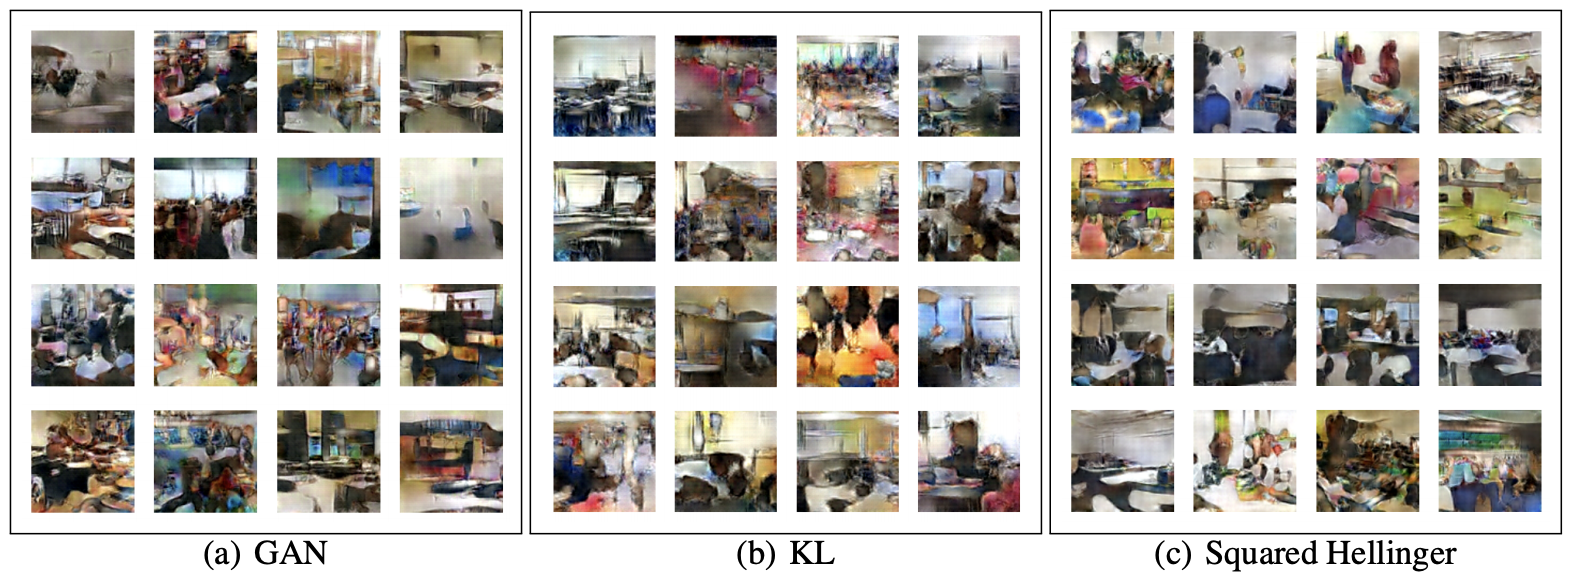
\includegraphics[width=1.0\linewidth]{figs/f_div_results}
	\end{figure}

	\myfootnotewithlink{https://arxiv.org/abs/1606.00709}{Nowozin S., Cseke B., Tomioka R. f-GAN: Training Generative Neural Samplers using Variational Divergence Minimization, 2016}
\end{frame}
%=======
\begin{frame}{Evaluation of likelihood-free models}
	How to evaluate generative models?
	\begin{block}{Likelihood-based models}
		\begin{itemize}
			\item Split data to train/val/test.
			\item Fit model on the train part.
			\item Tune hyperparameters on the validation part.
			\item Evaluate generalization by reporting likelihoods on the test set.
		\end{itemize}
	\end{block}
	\begin{block}{Not all models have tractable likelihoods}
		\begin{itemize}
			\item VAE: compare ELBO values.
			\item GAN: ???
		\end{itemize}
	\end{block}
\end{frame}
%=======
\begin{frame}{Evaluation of likelihood-free models}
	Let take some pretrained image classification model to get the conditional label distribution $p(y | \bx)$ (e.g. ImageNet classifier).
	\begin{block}{What do we want from samples?}
		\begin{itemize}
			\item \textbf{Sharpness}
			\begin{figure}
				\centering
				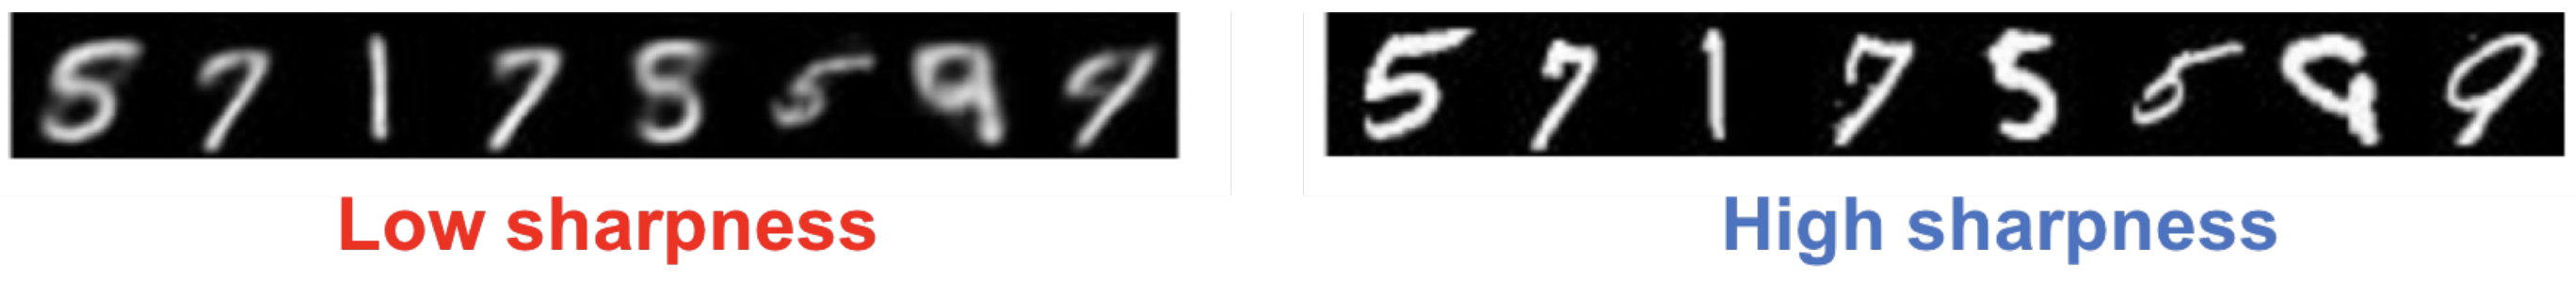
\includegraphics[width=0.9\linewidth]{figs/sharpness}
			\end{figure}
			The conditional distribution $p(y | \bx)$ should have low entropy (each image $\bx$ should have distinctly recognizable object).
			\item \textbf{Diversity}
			\begin{figure}
				\centering
				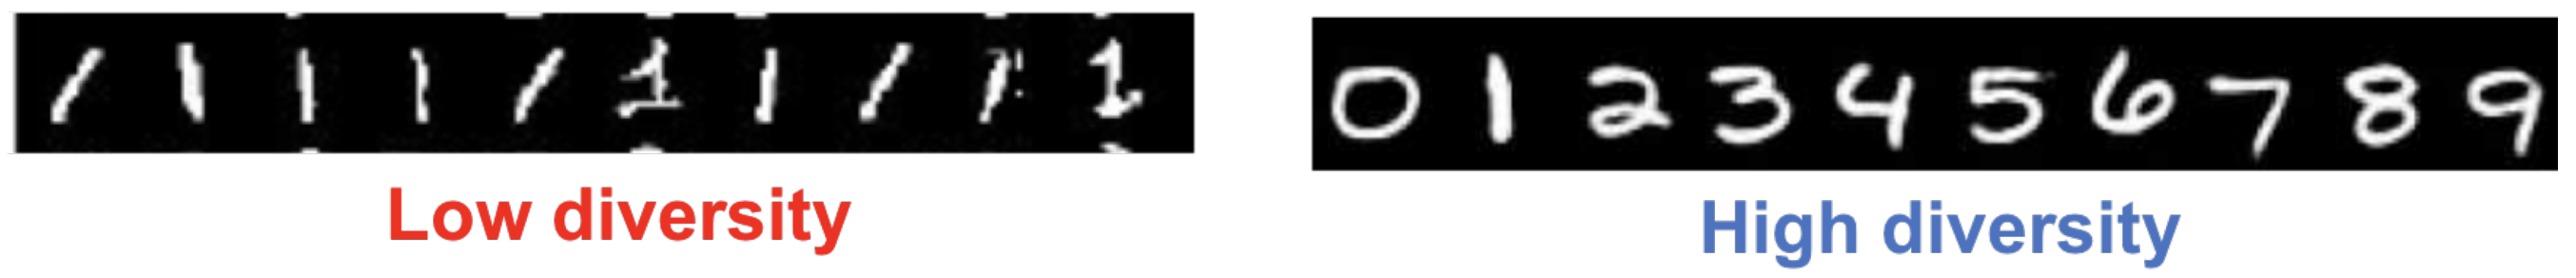
\includegraphics[width=0.9\linewidth]{figs/diversity}
			\end{figure}
			The marginal distribution $p(y) = \int p(y | \bx) p(\bx) d \bx$ should have high entropy (there should be as many classes generated as possible).
		\end{itemize}
	\end{block}
	\myfootnotewithlink{https://deepgenerativemodels.github.io}{image credit: https://deepgenerativemodels.github.io}
\end{frame}
%=======
\begin{frame}{Evaluation of likelihood-free models}
	\begin{block}{What do we want from samples?}
		\begin{itemize}
			\item \textbf{Sharpness.}
			The conditional distribution $p(y | \bx)$ should have low entropy (each image $\bx$ should have distinctly recognizable object).
			\item \textbf{Diversity.}
			The marginal distribution $p(y) = \int p(y | \bx) p(\bx) d \bx$ should have high entropy (there should be as many classes generated as possible).
		\end{itemize}
	\end{block}
	\begin{figure}
		\centering
		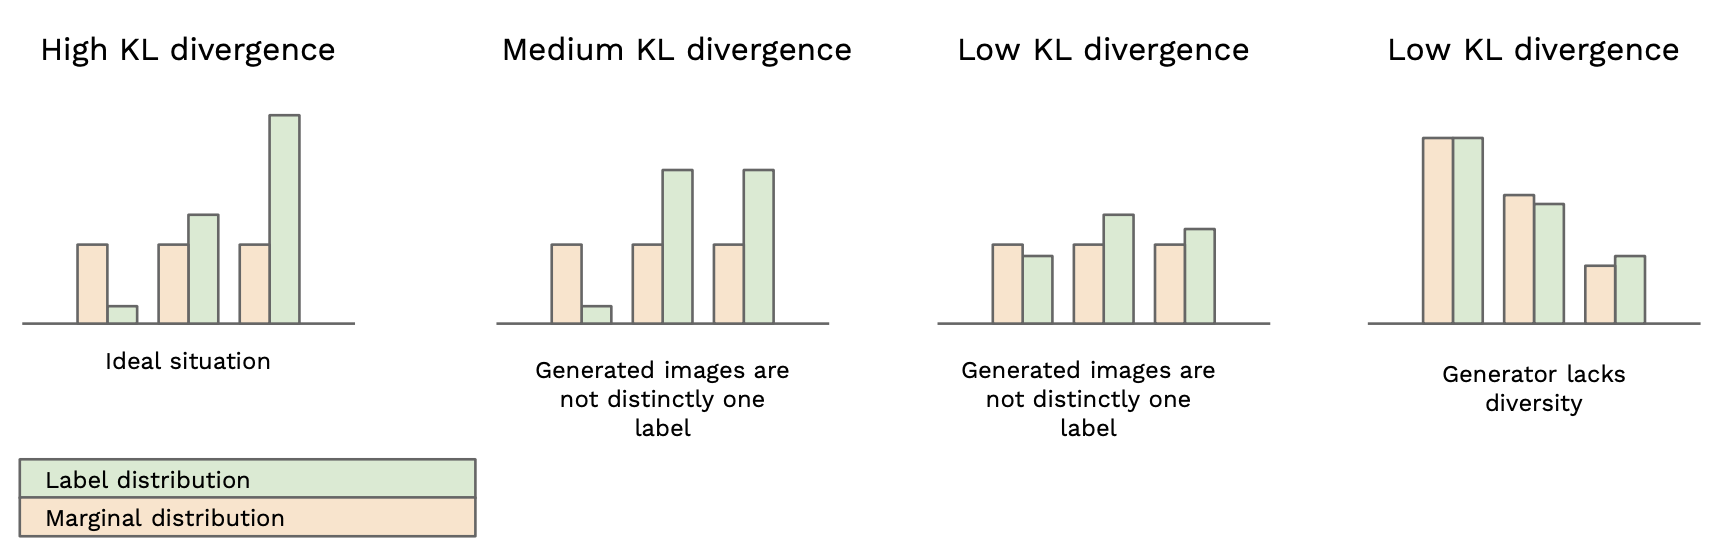
\includegraphics[width=1.0\linewidth]{figs/is_toy}
	\end{figure}
	\myfootnotewithlink{https://medium.com/octavian-ai/a-simple-explanation-of-the-inception-score-372dff6a8c7a}{image credit: https://medium.com/octavian-ai/a-simple-explanation-of-the-inception-score-372dff6a8c7a}
\end{frame}
%=======
\begin{frame}{Evaluation of likelihood-free models}
		\begin{block}{What do we want from samples?}
		\begin{itemize}
			\item Sharpness $\Rightarrow$ low $H(y | \bx) = - \sum_{y} \int_{\bx} p(y, \bx) \log p(y | \bx) d\bx$.
			\item Diversity $\Rightarrow$ high $H(y)  = - \sum_{y} p(y) \log p(y)$.
		\end{itemize}
	\end{block}
	\begin{block}{Inception Score}
		\vspace{-0.3cm}
		\footnotesize
		\begin{align*}
			IS &= \exp(H(y) - H(y | \bx)) \\ 
			&= \exp \left( - \sum_{y} p(y) \log p(y) + \sum_{y} \int_{\bx} p(y, \bx) \log p(y | \bx) d\bx\right) \\
			&= \exp \left( \sum_{y} \int_{\bx} p(y, \bx) \log \frac{p(y | \bx)}{p(y)} d\bx\right) \\ 
			&= \exp \left( \bbE_{\bx} \sum_{y} p(y | \bx) \log \frac{p(y | \bx)}{p(y)} \right) = \exp \left( \bbE_{\bx} KL(p(y | \bx) || p(y)) \right)
		\end{align*}
	\end{block}
	\myfootnotewithlink{https://arxiv.org/abs/1606.03498}{Salimans T. et al. Improved Techniques for Training GANs, 2016}
\end{frame}
%=======
\begin{frame}{Evaluation of likelihood-free models}
	\begin{block}{Inception Score}
		\vspace{-0.1cm}
		\[
			IS =  \exp \left( \bbE_{\bx} KL(p(y | \bx) || p(y)) \right)
		\]
		\vspace{-0.1cm}
	\end{block}
	\begin{block}{IS limitations}
		\begin{itemize}
			\item Inception score depends on the quality of the pretrained classifier $p(y | \bx)$.
			\item If generator produces images with a different set of labels from the classifier training set, IS will be low.
			\item If the generator produces one image per class, the IS will be perfect (there is no measure of intra-class diversity).
			\item IS only require samples from the generator and do not take into account the desired data distribution $\pi(\bx)$ directly (only implicitly via a classifier).
		\end{itemize}
	\end{block}
	\myfootnotewithlink{https://arxiv.org/abs/1801.01973}{Barratt S., Sharma R. A Note on the Inception Score, 2018}
\end{frame}
%=======
\begin{frame}{Evaluation of likelihood-free models}
	\begin{block}{Theorem}
		If $\pi(\bx)$ and $p(\bx | \btheta)$ has moment generation functions then
		\[
			\pi(\bx) = p(\bx | \btheta) \, \Leftrightarrow \, \bbE_{\pi} \bx^k = \bbE_{p} \bx^k, \quad \forall k \geq 1.
		\]
	\end{block}
	This is intractable to calculate all moments.
	\begin{block}{Frechet Inception Distance}
		\vspace{-0.1cm}
		\[
			D^2 (\pi, p) = \| \mathbf{m}_{\pi} - \mathbf{m}_{p}\|_2^2 + \text{Tr} \left( \bC_{\pi} + \bC_p - 2 \sqrt{\bC_{\pi} \bC_p} \right)
		\]
	\end{block}
	\begin{itemize}
		\item $\mathbf{m}_{\pi}$, $\bC_{\pi} $ are mean vector and covariance matrix of feature representations for real samples from $\pi(\bx)$
		\item $\mathbf{m}_{p}$, $\bC_p$ are mean vector and covariance matrix of feature representations for generated samples from $p(\bx | \btheta)$.
		\item Representations are outputs of intermediate layer from pretrained classification model.
	\end{itemize} 

	\myfootnotewithlink{https://arxiv.org/abs/1706.08500}{Heusel M. et al. GANs Trained by a Two Time-Scale Update Rule Converge to a Local Nash Equilibrium, 2017}
\end{frame}
%=======
\begin{frame}{Evaluation of likelihood-free models}
	\begin{figure}
		\centering
		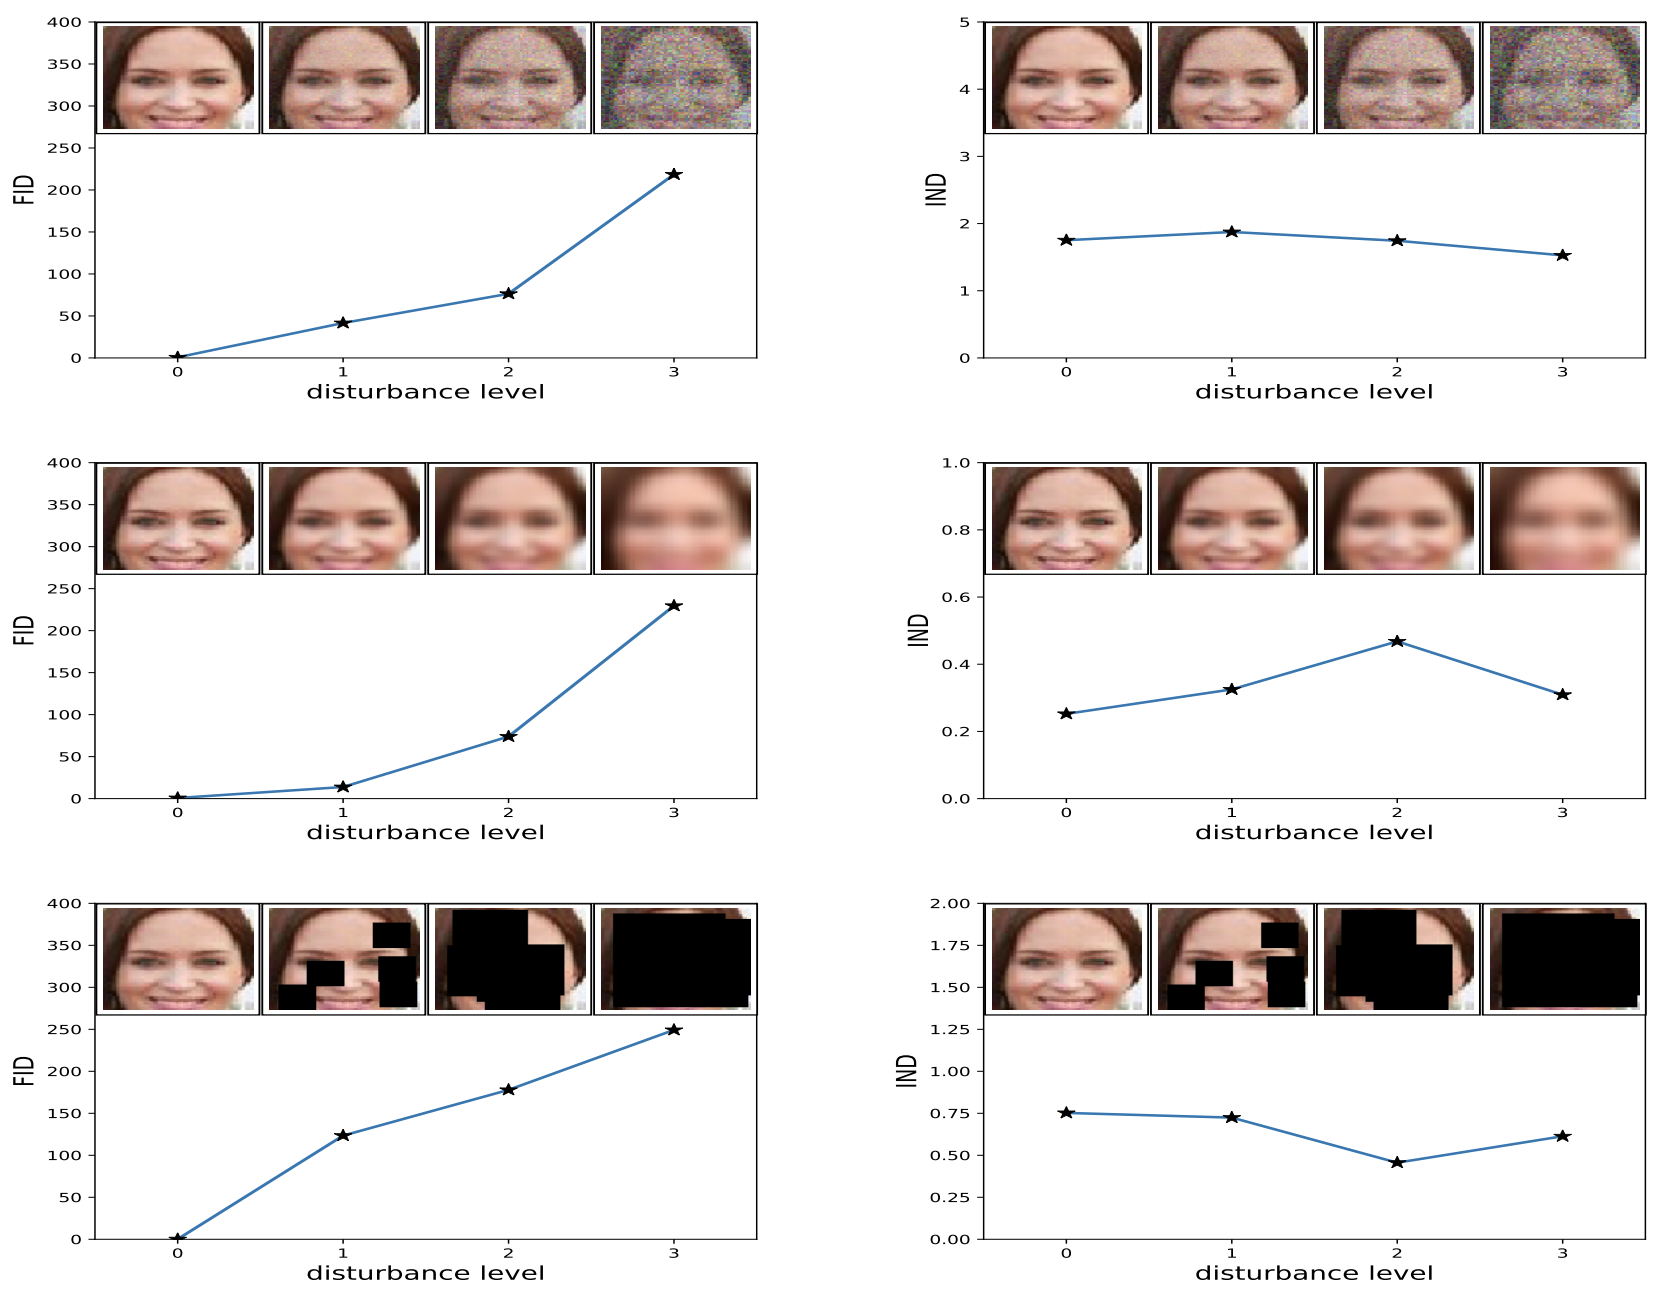
\includegraphics[width=0.9\linewidth]{figs/fid_results}
	\end{figure}
	
	\myfootnotewithlink{https://arxiv.org/abs/1706.08500}{Heusel M. et al. GANs Trained by a Two Time-Scale Update Rule Converge to a Local Nash Equilibrium, 2017}
\end{frame}
%=======
\begin{frame}{Evaluation of likelihood-free models}
	\begin{block}{Frechet Inception Distance}
		\vspace{-0.1cm}
		\[
		D^2 (\pi, p) = \| \mathbf{m}_{\pi} - \mathbf{m}_{p}\|_2^2 + \text{Tr} \left( \bC_{\pi} + \bC_p - 2 \sqrt{\bC_{\pi} \bC_p} \right)
		\]
	\end{block}
	\begin{block}{FID limitations}
		\begin{itemize}
			\item FID depends on the pretrained classification model.
			\item FID needs a large samples  size for evaluation.
			\item Calculation of FID is slow.
			\item FID extimates only two sample moments.
		\end{itemize}
	\end{block}

	\myfootnotewithlink{https://arxiv.org/abs/1706.08500}{Heusel M. et al. GANs Trained by a Two Time-Scale Update Rule Converge to a Local Nash Equilibrium, 2017}
\end{frame}
%=======
\begin{frame}{Summary}
	\begin{itemize}
		\item Wasserstein GAN uses Kantorovich-Rubinstein duality to estimate Wasserstein distance.
		\item Gradient Penalty proposes the regularizer to enforce Lipschitzness.
		\item Spectral normalization is a weight normalization technique to enforce Lipshitzness.
		\item f-divergence family is a unified framework for divergence minimization.
		\item Inception Score and Frechet Inception Distance are the common metrics for GAN evaluation.
	\end{itemize}
\end{frame}
%=======
\begin{frame}{Summary}
\end{frame}
%=======
\end{document} 